\documentclass[a4paper,12pt]{article}
\usepackage[top=3cm,right=2cm,bottom=2cm,left=3cm,a4paper]{geometry}
\usepackage[utf8]{inputenc}
\usepackage[brazil]{babel}
\usepackage{graphicx}
\usepackage{amsmath}
\usepackage{xcolor}
\usepackage{url}
\usepackage{enumitem}
\usepackage{float}
\usepackage{eso-pic}
\usepackage{fancyhdr}
\usepackage{lastpage}
\usepackage{lipsum, mlmodern}
\usepackage{hyperref}
\usepackage{indentfirst}
\usepackage{tabularx}

\setlength{\headheight}{15pt}

\pagestyle{fancy}
\fancyhf{}

% Cabeçalho
\fancyhead[L]{IFSC - ADS - Damares Gaia, Eduardo Cardoso e Talles Souza}
\fancyhead[C]{}
\fancyhead[R]{}

% Rodapé
\fancyfoot[L]{Documento produzido em \LaTeX} 
\fancyfoot[C]{}
\fancyfoot[R]{Página \thepage\ de \pageref{LastPage}}
\renewcommand{\footrulewidth}{0.4pt}

\setlength{\parindent}{0em}
\setlength{\parskip}{0em}

\begin{document}

\begin{titlepage}
\thispagestyle{empty}
\noindent
\centering
\vspace*{3cm}


\includegraphics[width=0.25\linewidth]{Imagens/IFSC_logo_vertical.png}
\vspace{2cm}

{\Huge \textbf{Projeto Final - Engenharia de Software I} \par}
\vspace{1cm}

{\large \textit{Assistente de cultivo doméstico} \par}
\vfill

{\large Damares, Eduardo e Talles, 2026 \par}
\vspace{0.5cm}
    
\end{titlepage} \newpage

% =========================================================================
% SEÇÃO 1 - PROCESSO DE SOFTWARE
% =========================================================================
\section{Processo de Software}

Para o desenvolvimento do \textit{Assistente de Cultivo Doméstico}, a equipe optou por um fluxo de processo iterativo, no qual as fases metodológicas podem ser revisitadas e ajustadas ciclicamente ao longo do projeto. Como suporte operacional a este fluxo, foi adotada a metodologia ágil Scrum. 

Esta escolha justifica-se pelo facto de a agilidade promover uma resposta rápida, eficaz e adaptativa às mudanças de requisitos. O Scrum, especificamente, oferece um modelo flexível de trabalho ideal para equipes pequenas e projetos com prazos rígidos, garantindo a entrega rápida de incrementos funcionais de software.

\subsection{Organização e Papéis da equipe}
Em conformidade com os princípios de equipes ágeis auto-organizadas e com alta autonomia , os papéis foram divididos focando-se nos membros diretamente comprometidos com a construção e entrega do produto:

\begin{itemize}[leftmargin=*]
    \item \textbf{Product Owner (Damares Gaia):} Responsável por gerir e priorizar o \textit{Product Backlog}, alinhando os cenários desejados com as necessidades de negócio do ecossistema de cultivo.
    \item \textbf{Scrum Master (Talles Souza):} Atua como o líder do processo, responsável por garantir a aderência às práticas do framework, remover impedimentos técnicos e facilitar o fluxo de trabalho da equipe.
    \item \textbf{Time de Desenvolvimento (Eduardo, Damares e Talles):} equipe técnica autogerida encarregue de projetar a arquitetura, desenhar os diagramas de modelagem, codificar a aplicação e implementar o plano de testes.
\end{itemize}

\subsection{Dinâmica de Trabalho e Cerimónias}
O ciclo de desenvolvimento foi estruturado em \textit{Sprints} de uma semana. A dinâmica operacional do grupo engloba as seguintes práticas fundamentais:
\begin{itemize}[leftmargin=*]
    \item \textbf{Planeamento do Sprint (\textit{Sprint Planning}):} Reunião realizada no início de cada ciclo para refinar o \textit{Product Backlog} e selecionar os itens prioritários que farão parte do \textit{Sprint Backlog} da semana.
    \item \textbf{Reunião Diária (\textit{Daily Scrum}):} Encontros de alinhamento com duração estrita de 15 minutos. Cada membro responde brevemente a três perguntas essenciais: o que foi feito desde o último encontro, o que será feito no dia corrente e se existe algum impedimento que bloqueie o progresso.
    \item \textbf{Revisão do Sprint (\textit{Sprint Review}):} Sessão realizada ao fecho de cada iteração para demonstrar o incremento de software em modo texto desenvolvido e recolher avaliações críticas da equipe.
\end{itemize}

\vspace{2em}

% =========================================================================
% SEÇÃO 2 - REQUISITOS DE SOFTWARE
% =========================================================================
\section{Requisitos de Software}

A especificação do sistema foi detalhada por meio da identificação de requisitos funcionais e não funcionais, mapeados sob a forma de Histórias de Usuário para guiar o desenvolvimento iterativo focado no valor prático da aplicação. Dado que o sistema será executado exclusivamente via Interface de Linha de Comando (CLI) no terminal, o escopo foi projetado para assegurar robustez textual.

\subsection{Requisitos Funcionais (RF)}
Os requisitos funcionais determinam as ações, recursos e comportamentos que o sistema de terminal deve fornecer:
\begin{enumerate}[label=\textbf{RF\arabic*}]
    \item O sistema deve disponibilizar um menu principal interativo em modo texto para navegação do utilizador.
    \item O sistema deve permitir que o utilizador registe as suas plantas via console, solicitando dados como espécie, apelido e data de aquisição.
    \item O sistema deve manter uma base de dados local (armazenada em memória ou ficheiro de texto) com os parâmetros de rega, adubação e poda de diferentes espécies.
    \item O sistema deve calcular e imprimir no ecrã a listagem de alertas de cuidados pendentes de forma automática assim que o programa for iniciado.
    \item O sistema deve permitir o registo manual de atividades (como a realização de uma rega ou poda) num diário de cultivo.
    \item O sistema deve ser capaz de imprimir uma tabela estruturada no terminal exibindo o estado de saúde e o histórico de todas as plantas cadastradas.
\end{enumerate}

\subsection{Requisitos Não Funcionais (RNF)}
Os requisitos não funcionais especificam restrições arquiteturais e critérios de qualidade do software:
\begin{enumerate}[label=\textbf{RNF\arabic*}]
    \item \textbf{Usabilidade em CLI:} A interface de texto deve ser amigável, provendo menus numéricos claros, validação estrita de dados de entrada e tratamento de exceções para evitar interrupções abruptas do programa por falhas de digitação do utilizador.
    \item \textbf{Desempenho:} O tempo de processamento para exibição das listagens textuais e cálculo dos intervalos de manutenção não deve ultrapassar 1 segundo.
    \item \textbf{Portabilidade:} O programa deve ser independente de sistema operativo, sendo executável em qualquer interpretador de comandos padrão (Terminal Linux/macOS, PowerShell ou Prompt de Comando do Windows).
\end{enumerate}

\subsection{Histórias de Usuário (User Stories)}
As histórias traduzem os requisitos para o cenário prático do utilizador:
\begin{itemize}[leftmargin=*]
    \item \textbf{US01 -- Registo de Planta:} Como um entusiasta da jardinagem, eu quero digitar os dados das minhas plantas no terminal, para que o sistema armazene o histórico e recomende os cuidados adequados de acordo com a espécie (Atende ao \textbf{RF2}).
    \item \textbf{US02 -- Alertas de Cuidado:} Como um utilizador esquecido, eu quero visualizar um resumo textual de alertas de rega logo na inicialização do prompt, para não deixar as minhas plantas morrerem por dessecação (Atende ao \textbf{RF4}).
    \item \textbf{US03 -- Diário de Cultivo:} Como um cuidador de plantas, eu quero registar no histórico a data exata em que realizei uma rega, para monitorizar o ciclo de humidade e evitar o excesso de água (Atende ao \textbf{RF5}).
    \item \textbf{US04 -- Menu Interativo de Navegação:} Como um utilizador do sistema via terminal, eu quero navegar pelas funcionalidades através de um menu de texto interativo e numérico, para que eu possa aceder aos recursos do assistente de forma simples e intuitiva sem precisar de memorizar comandos complexos (Atende ao \textbf{RF1}).
    \item \textbf{US05 -- Consulta de Parâmetros por Espécie:} Como um botânico amador, eu quero que o sistema mantenha uma base de dados local com os parâmetros ideais de rega, adubação e poda de cada espécie, para que a aplicação calcule os alertas de cuidados com base em critérios biológicos fiáveis (Atende ao \textbf{RF3}).
    \item \textbf{US06 -- Painel Geral de Saúde e Histórico:} Como um cuidador focado na organização, eu quero visualizar uma tabela estruturada com o estado de saúde e o histórico completo de todas as minhas plantas registadas, para que eu tenha uma visão panorâmica e integrada do progresso do meu cultivo doméstico (Atende ao \textbf{RF6}).
\end{itemize}

\vspace{2em}

% =========================================================================
% SEÇÃO 3 - MODELO DE SOFTWARE
% =========================================================================
\section{Modelo de Software}

A modelagem do sistema estabelece o plano estrutural e comportamental que serve de roteiro para a construção correta do software. Foram elaborados os diagramas obrigatórios utilizando a Unified Modeling Language (UML), orientando o design técnico para uma arquitetura baseada em console.

\subsection{Diagrama de Casos de Uso}
O Diagrama de Casos de Uso expõe as fronteiras do sistema e como o ator (\textit{Utilizador}) interage ativamente com a aplicação através dos comandos disponíveis no terminal.

\begin{figure}[H]
    \centering
    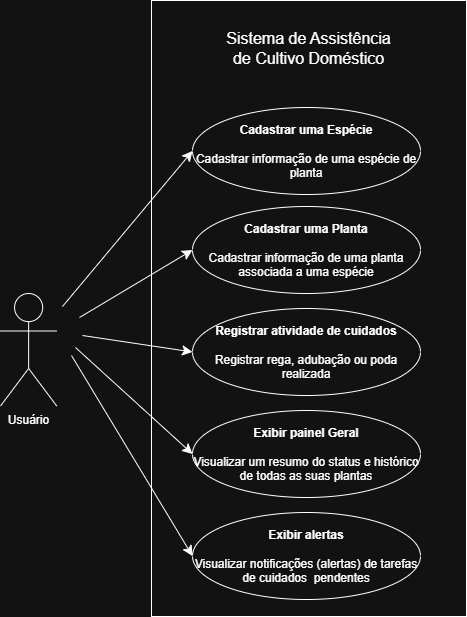
\includegraphics[width=0.6\textwidth]{Imagens/diagrama_casos_uso.png}
    \caption{Diagrama de Casos de Uso do Assistente CLI.}
    \label{fig:casos_uso}
\end{figure}

\subsection{Diagrama de Classes}
O Diagrama de Classes detalha a visão estática do domínio. Como o sistema não possui interface gráfica, evitou-se o acoplamento com bibliotecas visuais complexas. O fluxo de entrada e saída é gerido por uma classe controladora centralizada chamada \textbf{MenuPrompt}, que se comunica com as classes de entidade e negócio: \textbf{Usuario}, \textbf{Planta}, \textbf{Especie} e \textbf{RegistroDiario}.

\begin{figure}[H]
    \centering
    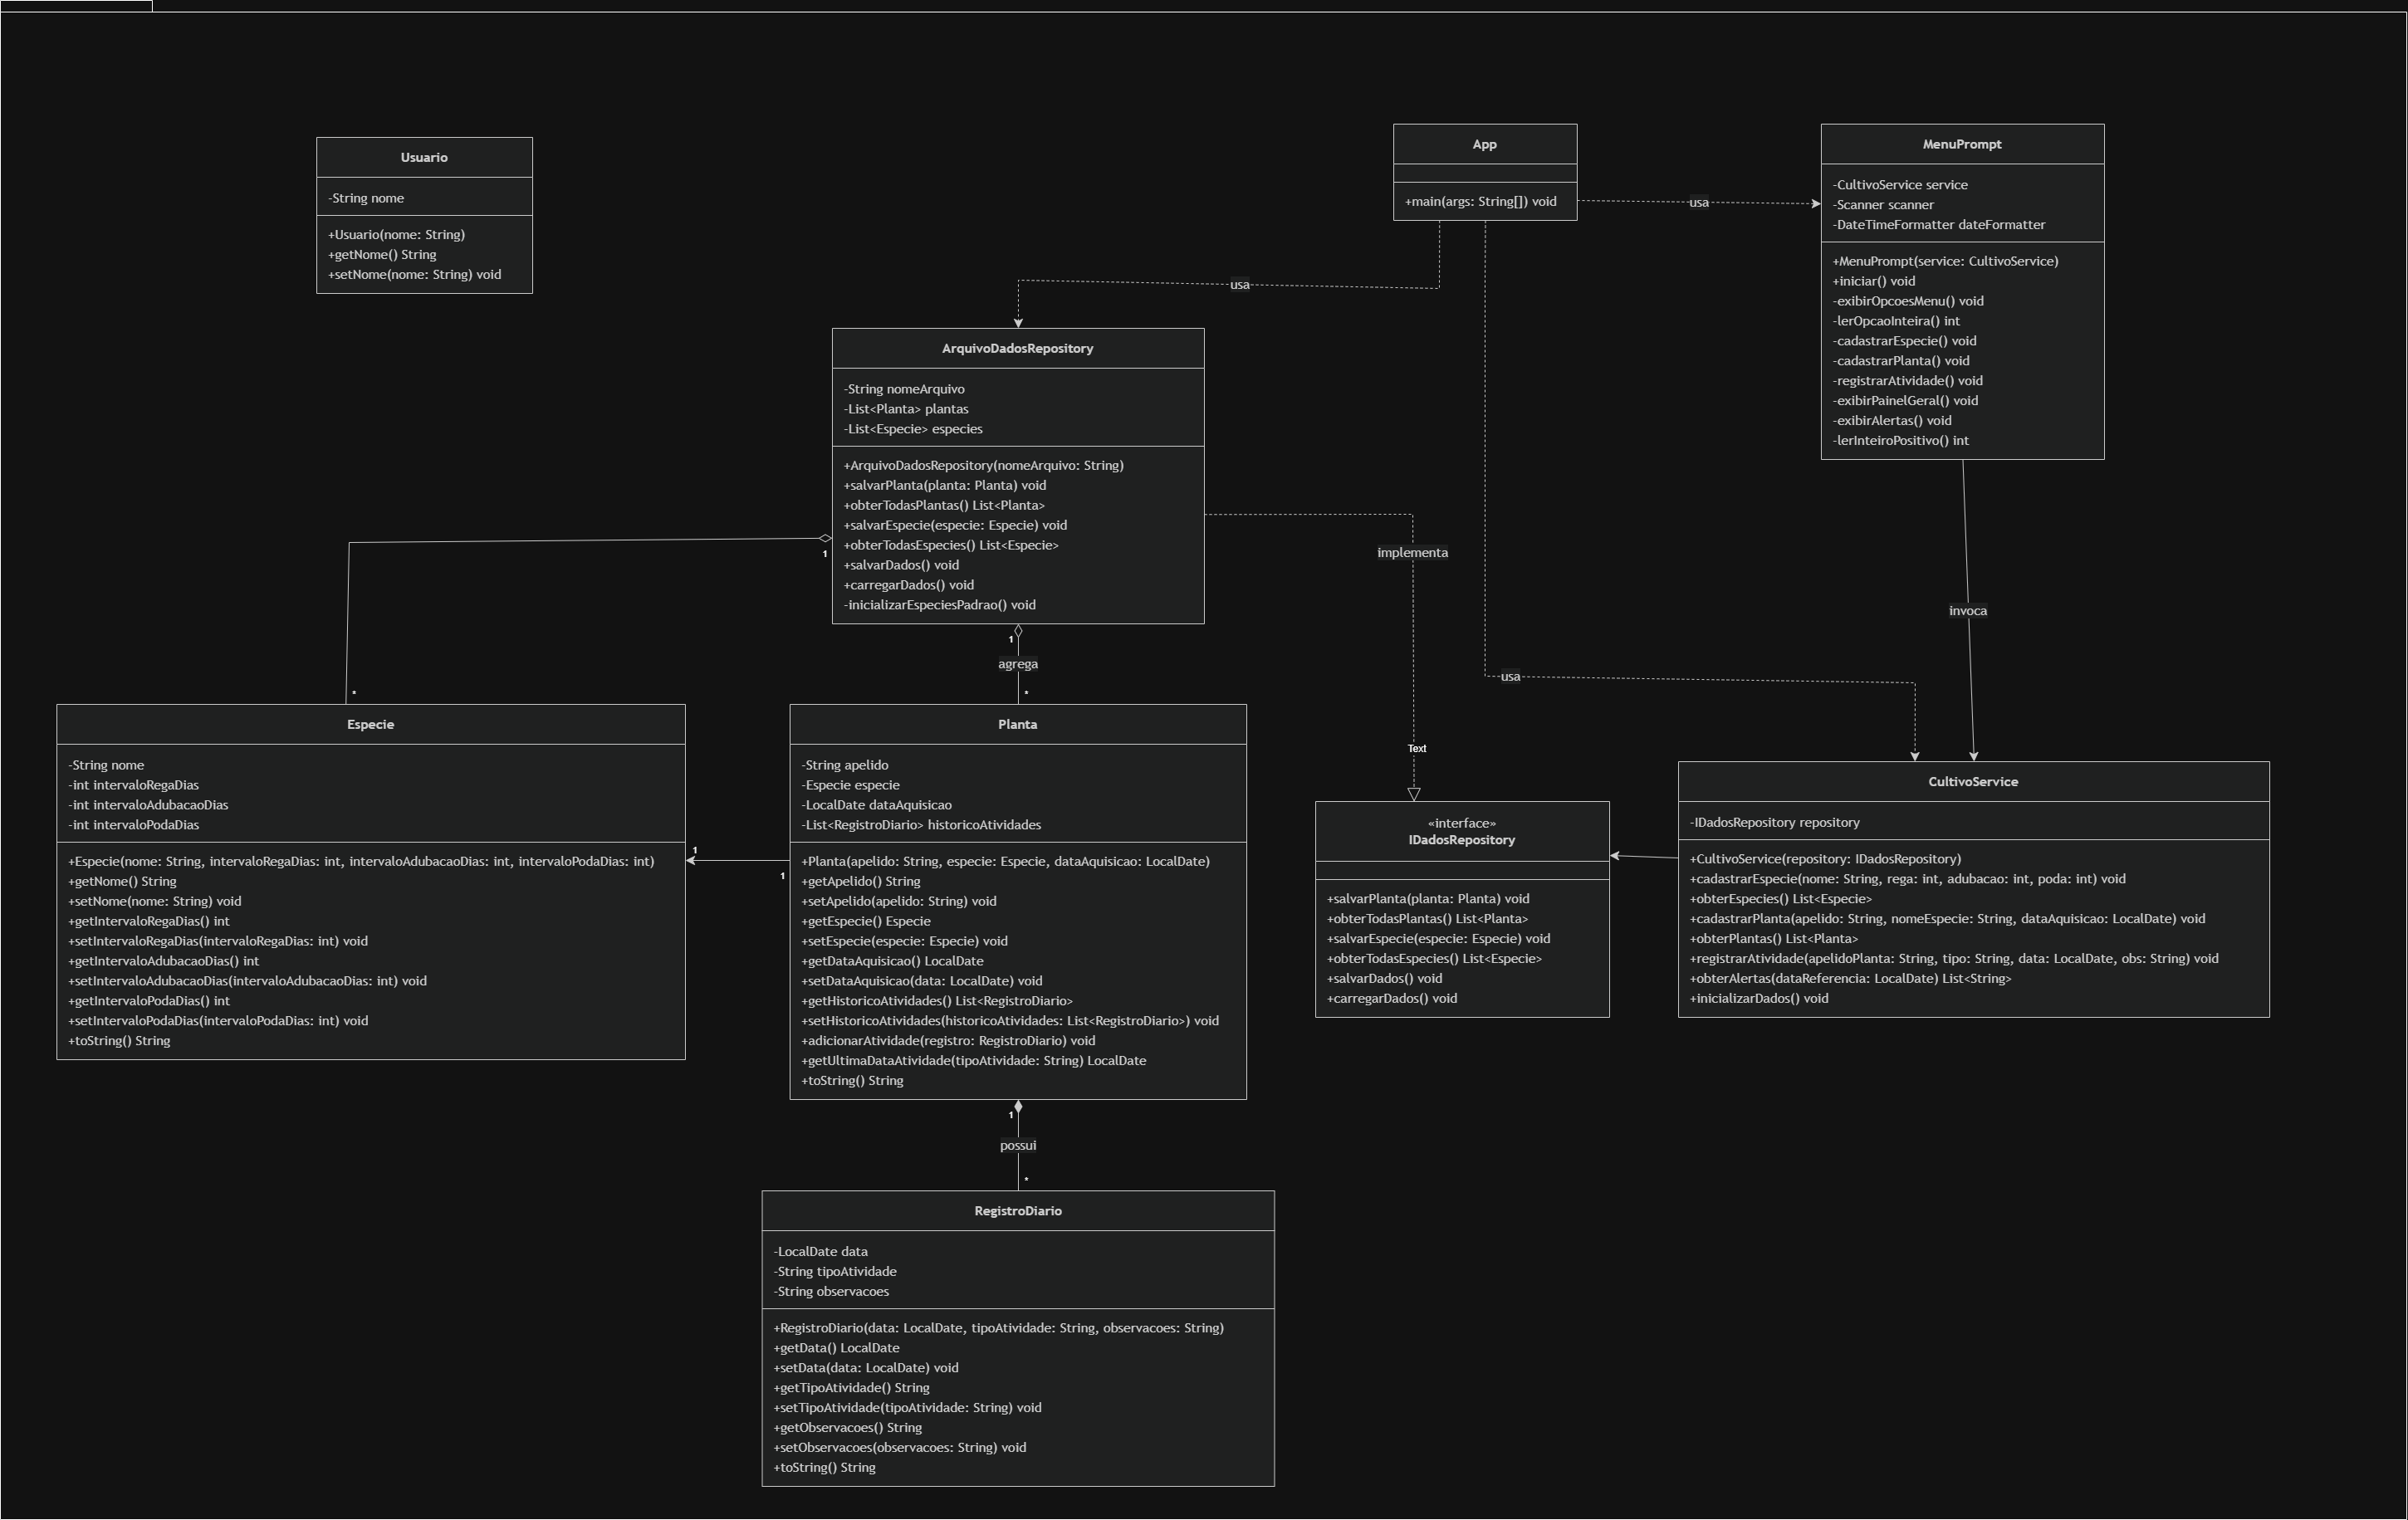
\includegraphics[width=\textwidth]{Imagens/diagrama_classes.png}
    \caption{Diagrama de Classes Orientado a Objetos.}
    \label{fig:classes}
\end{figure}

\subsection{Diagrama Dinâmico (Sequência)}
O Diagrama de Sequência mapeia a perspetiva dinâmica do software, ilustrando a troca de mensagens cronológica entre os objetos do sistema quando o utilizador solicita a listagem de plantas e o cálculo automático dos alertas de rega pendentes.

\begin{figure}[H]
    \centering
    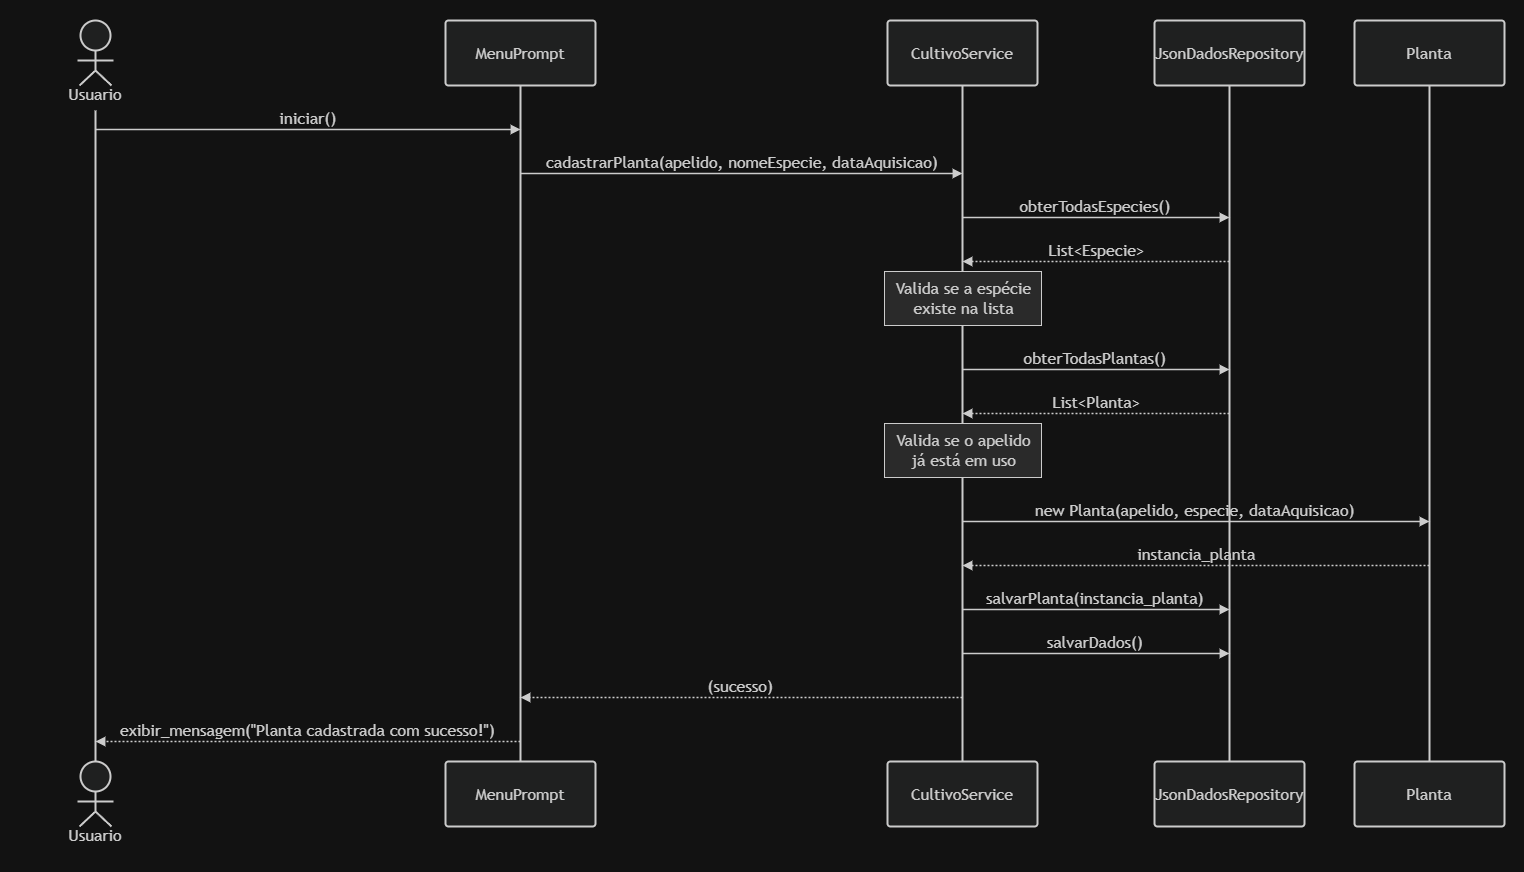
\includegraphics[width=0.85\textwidth]{Imagens/diagrama_sequencia.png}
    \caption{Diagrama de Sequência: Registrar Planta.}
    \label{fig:sequencia}
\end{figure}

\vspace{2em}

% =========================================================================
% SEÇÃO 4 - PRINCÍPIOS E PROPRIEDADES DE PROJETO
% =========================================================================
\section{Princípios e Propriedades de Projeto}

A organização arquitetural do assistente de cultivo seguiu princípios consolidados de engenharia para assegurar a manutenibilidade do código-fonte.

\begin{itemize}[leftmargin=*]
    \item \textbf{Integridade Conceitual:} O padrão estrutural do sistema é uniforme. Todas as classes seguem a mesma convenção de nomenclatura e separação de responsabilidades, garantindo harmonia no design abstrato da aplicação.
    \item \textbf{Coesão:} Cada componente possui uma responsabilidade única e bem delimitada. A classe \textit{MenuPrompt} restringe-se à captura e exibição de strings no console, enquanto a classe \textit{Planta} gerencia estritamente as regras de estado do vegetal.
    \item \textbf{Baixo Acoplamento:} A separação total entre as classes de negócio e o console gerou um acoplamento extremamente reduzido. Caso a equipe decida futuramente migrar a interface do terminal para uma aplicação móvel Android ou Web, a lógica central de cálculo de rega e os modelos de dados permanecerão intactos, sendo necessária apenas a substituição da camada de interface.
    \item \textbf{Ocultação de Informação:} Os atributos das classes de dados foram encapsulados com modificadores de acesso privados. A leitura e a modificação de variáveis sensíveis, como a data da última rega, dão-se obrigatoriamente através de métodos públicos controladores (\textit{Getters} e \textit{Setters}), impedindo estados inconsistentes.
    \item \textbf{Princípios SOLID:} A organização das classes e o fluxo de mensagens foram estruturados em conformidade com o acrónimo SOLID, blindando o software contra a rigidez e a fragilidade do código:
    \begin{itemize}[label=$\circ$, leftmargin=1.5em]
        \item \textit{Single Responsibility Principle (SRP):} Cada classe possui uma única razão para mudar. A classe controlador \textbf{MenuPrompt} é estritamente encarregue da captura e exibição de strings no console (apresentação), enquanto as classes de entidade como \textbf{Planta} e \textbf{Especie} gerem exclusivamente as regras biológicas de estado do vegetal e os dados botânicos, evitando o acoplamento caótico entre regras de negócio e a interface com o utilizador.
        \item \textit{Open/Closed Principle (OCP):} O sistema é aberto para extensão e fechado para modificação. O motor de cálculo de rotinas de alertas foi isolado através do modelo de composição. Caso surja a necessidade de implementar novas regras de cultivo futuras (como o cálculo de exposição solar ou controlo de ph do solo), novos comportamentos podem ser integrados anexando novas propriedades ao objeto composicional \textbf{Especie}, expandindo a aplicação sem alterar ou quebrar as rotinas de listagem estruturada já existentes.
        \item \textit{Liskov Substitution Principle (LSP):} Garante-se que as classes derivadas ou as implementações concretas possam substituir as suas abstrações base sem alterar a corretude do programa. Apesar de o domínio do sistema priorizar fortemente a composição sobre a herança para evitar acoplamento rígido, os contratos de persistência locais e os controladores de fluxo são desenhados para que qualquer substituição polimórfica opere perfeitamente sem gerar efeitos colaterais.
        \item \textit{Interface Segregation Principle (ISP):} O sistema evita a criação de interfaces ``gordas'' e genéricas. Os contratos e interfaces abstratas do assistente são cirurgicamente segregados e enxutos. Isso assegura que os módulos clientes (como a própria classe de interface CLI) não sejam forçados a depender ou a implementar métodos de baixo nível de escrita física em disco dos quais não fazem uso direto.
        \item \textit{Dependency Inversion Principle (DIP):} Os módulos de alto nível (a lógica de negócio do ecossistema de cultivo) não dependem de módulos de baixo nível (mecanismos concretos de ficheiros de texto ou escrita em disco). Ambas as camadas dependem de abstrações intermédias através de uma interface de persistência de dados. Essa inversão de dependência isolou o núcleo da aplicação e permitiu o desacoplamento seguro que viabilizou a criação dos objetos simulados (\textit{Mocks}) no ecossistema de testes unitários do projeto.
    \end{itemize}
    \item \textbf{Preferência por Composição em vez de Herança:} Para evitar hierarquias rígidas e complexas de classes, utilizou-se a composição. Uma \textit{Planta} não herda de um tipo biológico específico; ela ``tem um'' objeto do tipo \textit{Especie}, o que confere maleabilidade para atribuir novos perfis botânicos dinamicamente.
    \item \textbf{Lei de Demeter:} O código foi estruturado para que as classes interajam apenas com dependências diretas. Métodos de objetos terceiros obtidos por intermédio de acessores encadeados não são invocados, limitando o impacto de modificações internas em cadeia.
\end{itemize}

\vspace{2em}

% =========================================================================
% SEÇÃO 5 - TESTES DE SOFTWARE
% =========================================================================
\section{Testes de Software}

A estratégia de verificação do projeto consistiu no planeamento de testes automatizados para atestar a precisão lógica das regras de negócio e o comportamento seguro do sistema sob condições de erro.

\subsection{Testes Unitários}
A ausência de uma interface gráfica complexa viabilizou o isolamento completo da lógica de dados para testes. Foram escritos testes unitários focados nas seguintes componentes críticas do sistema:
\begin{itemize}[leftmargin=*]
    \item \textbf{Validação do Motor de Rega:} Testes automatizados que injetam diferentes históricos de datas para certificar que o cálculo do intervalo de dias para a próxima rega não resulta em valores negativos ou inconsistências de calendário.
    \item \textbf{Tratamento de Exceções de Entrada:} Testes concebidos para avaliar se os validadores de texto do terminal respondem corretamente quando o utilizador digita caracteres inválidos ou valores nulos em campos numéricos do menu.
\end{itemize}

\subsection{Uso de Mocks}
Para isolar o comportamento de unidades específicas e neutralizar dependências externas complexa, foram arquitetados objetos simulados (\textit{Mocks}):
\begin{itemize}[leftmargin=*]
    \item \textbf{\textit{Mock} de Persistência de Dados:} Simulação da camada de armazenamento local. Este objeto mockado intercepta as chamadas de salvamento, gravando as plantas temporariamente em listas de memória volátil, o que permite testar a criação de diários sem realizar operações reais de leitura e escrita em ficheiros de texto durante a execução dos testes.
    \item \textbf{\textit{Mock} de Emissão de Alertas:} Objeto que simula o disparo de gatilhos de atenção, permitindo inspecionar se os métodos internos agendam os avisos de adubação e rega nos prazos corretos, sem depender do envio físico de saídas de texto para o console do sistema operativo.
\end{itemize}

\end{document}